\section{Rb 05A}
The Rb 05A is a remote-controlled missile.
It is primarily intended for use against ground and naval targets,
but can also be used against slow-manoeuvring air targets thanks to a proximity fuse.
The missile is guided visually by the pilot.
A flare at the back of the missile helps the pilot to keep sight of it (\cref{fig:rb05-flare}).

\begin{figure}
  \centering
  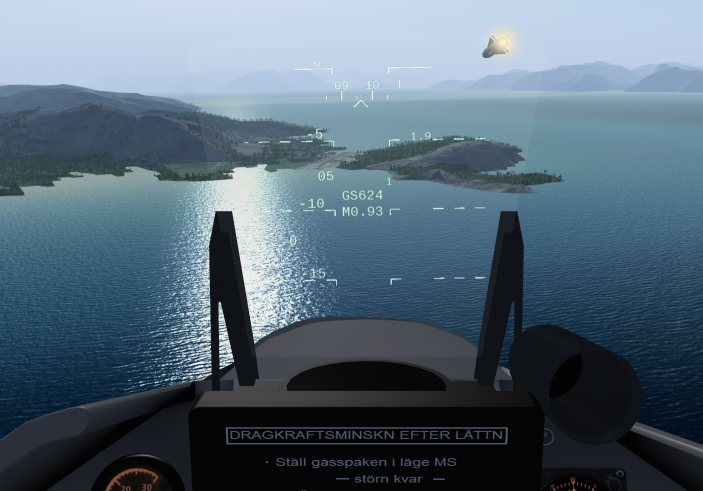
\includegraphics[height=0.3\textwidth]{images/weapons/rb_05a_start_popup.png}
  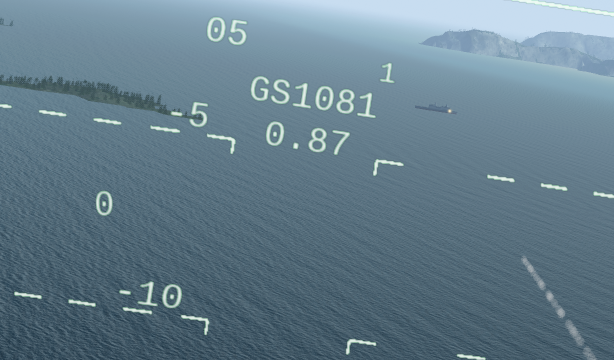
\includegraphics[height=0.3\textwidth]{images/weapons/rb_05a_before_impact_ship.png}
  \caption[Rb 05A flare for visual guidance]{Rb 05A flare for visual guidance.
    On the left, the missile is entering the pilot's field of view just after launch.
    On the right, the missile is about to hit the target ship,
    and the missile flare is visible over the ship
  }
  \label{fig:rb05-flare}
\end{figure}

In FlightGear, the Rb 05A uses the same controls as the radar stick, cf.\ \cref{sec:cursor}.\footnote{%
  In the real Viggen, a separate control stick on the right console was used.
}

\subsection{Procedure}
\begin{enumerate}
  \item Main mode selector to ANF/CBT.
    (\cockpitref{fig:left-panel}{item:main-mode}, shortcuts \keys{M}/\keys{\shift+M}).
  \item Select the Rb 05A (cycle weapons with \keys{C}).
  \item Once in firing position, consider engaging autopilot in ATT or HÖJD/ALT mode to reduce pilot workload.
  \item Identify the target visually.
  \item Unsafe the trigger and fire within 9km of the target.
  \item After 1.7s, missile controls are enabled
    (cf.\ \cref{sec:cursor} for control methods).
    At this point, it should be well within the pilot field of view.
  \item When the missile hits, take evasive manoeuvres, secure the trigger, and switch to NAV mode.
\end{enumerate}

Remarks.
\begin{itemize}
  \item Recommended speed is 700-1150 km/h.
  \item Recommended attitude is a level flight or slight dive,
    so as to not loose sight of the target and the missile.
  \item Recommended altitude is 300-400 meters above ground.
  \item The target do not need to be directly in front of the aircraft
    as the missile can be guided considerably to the side.
    However, doing so makes it harder to aim the missile, and reduces effective range.
  \item The missile flies for ca.\ 24 seconds, giving it a maximum effective range of ca.\ 9 km.
  \item It is easiest to aim the missile using the collimation principle:
    try to keep the missile flare covering the target at all time.
\end{itemize}
